\documentclass[border=10pt]{standalone}
\usepackage[T1]{fontenc}
\usepackage{tikz}
\usetikzlibrary{positioning, arrows.meta, shapes.geometric, fit, calc}

\definecolor{llmfill}{HTML}{D9D9D9}
\definecolor{procfill}{HTML}{F0F0F0}
\definecolor{iofill}{HTML}{E8E8E8}
\definecolor{sefill}{HTML}{BFBFBF}
\definecolor{edgecol}{HTML}{333333}

\tikzset{
    every node/.style={font=\sffamily\small},
    process/.style={
        rectangle, rounded corners=3pt, draw=edgecol, line width=0.8pt,
        fill=procfill, minimum width=3.2cm, minimum height=1cm,
        align=center,
    },
    llmcall/.style={
        process, fill=llmfill,
    },
    decision/.style={
        diamond, draw=edgecol, line width=0.8pt, fill=white,
        aspect=2, minimum width=2.5cm, inner sep=1pt, align=center,
    },
    startend/.style={
        rectangle, rounded corners=8pt, draw=edgecol, line width=1pt,
        fill=sefill, minimum width=2.2cm, minimum height=0.7cm,
        align=center, font=\sffamily\small\bfseries,
    },
    io/.style={
        rectangle, rounded corners=2pt, draw=edgecol!50, line width=0.5pt,
        fill=iofill, font=\sffamily\scriptsize, align=center,
    },
    arr/.style={-{Stealth[length=5pt]}, edgecol, line width=0.8pt},
    arrio/.style={-{Stealth[length=4pt]}, edgecol!50, line width=0.5pt},
    lbl/.style={font=\sffamily\scriptsize, text=edgecol!80},
}

\begin{document}
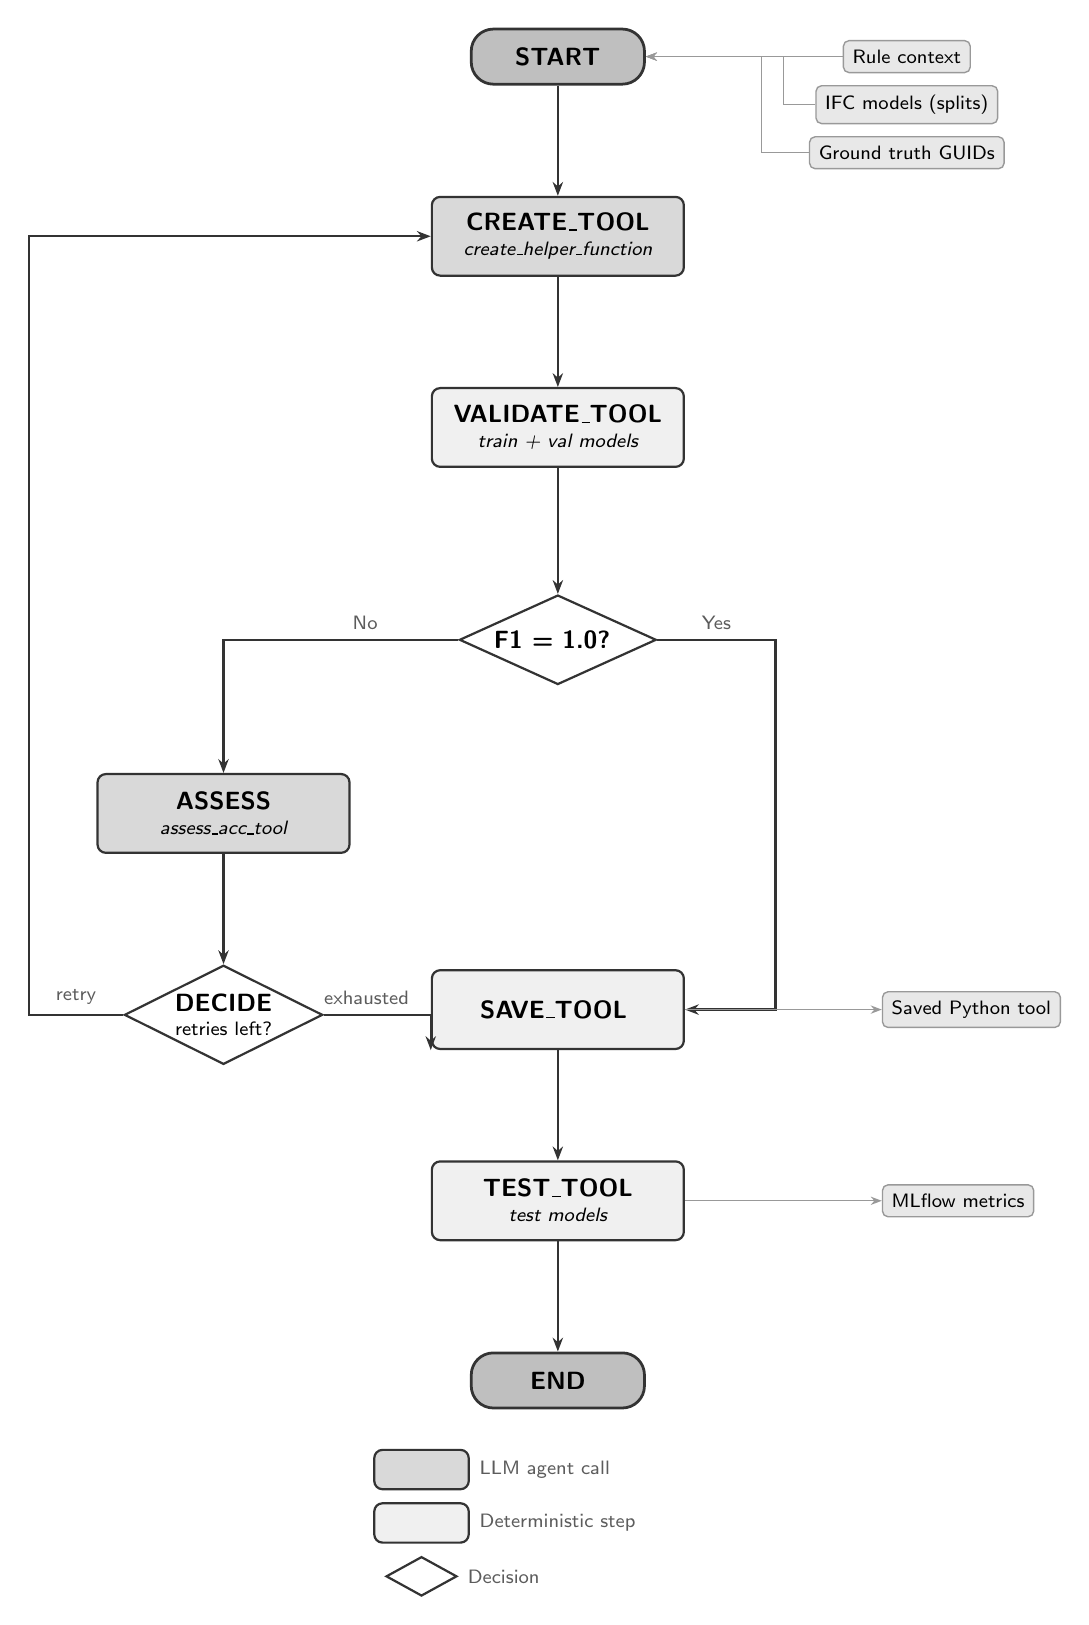
\begin{tikzpicture}[node distance=1.4cm]

% ── Nodes ──────────────────────────────────────────────────────────
\node[startend] (start) {START};

\node[llmcall, below=of start] (create) {
    \textbf{CREATE\_TOOL}\\[-2pt]
    {\scriptsize\itshape create\_helper\_function}
};

\node[process, below=of create] (validate) {
    \textbf{VALIDATE\_TOOL}\\[-2pt]
    {\scriptsize\itshape train + val models}
};

\node[decision, below=1.6cm of validate] (f1check) {
    \textbf{F1 = 1.0?}
};

\node[llmcall, below left=1.4cm and 2cm of f1check] (assess) {
    \textbf{ASSESS}\\[-2pt]
    {\scriptsize\itshape assess\_acc\_tool}
};

\node[decision, below=1.4cm of assess] (decide) {
    \textbf{DECIDE}\\[-2pt]
    {\scriptsize retries left?}
};

\node[process, below=3.6cm of f1check] (save) {
    \textbf{SAVE\_TOOL}
};

\node[process, below=of save] (test) {
    \textbf{TEST\_TOOL}\\[-2pt]
    {\scriptsize\itshape test models}
};

\node[startend, below=of test] (end) {END};

% ── Straight edges ─────────────────────────────────────────────────
\draw[arr] (start) -- (create);
\draw[arr] (create) -- (validate);
\draw[arr] (validate) -- (f1check);
\draw[arr] (save) -- (test);
\draw[arr] (test) -- (end);

% ── F1 = 1.0? → Yes → SAVE (right) ───────────────────────────────
\draw[arr] (f1check.east) -- ++(1.5,0) node[lbl, above, midway] {Yes}
           |- (save.east);

% ── F1 = 1.0? → No → ASSESS (left) ──────────────────────────────
\draw[arr] (f1check.west) -| (assess.north)
    node[lbl, above left, pos=0.15] {No};

% ── ASSESS → DECIDE ──────────────────────────────────────────────
\draw[arr] (assess) -- (decide);

% ── DECIDE → retry → CREATE_TOOL (loop left) ─────────────────────
\draw[arr] (decide.west) -- ++(-1.2,0)
    node[lbl, above, midway] {retry}
    |- (create.west);

% ── DECIDE → exhausted → SAVE ────────────────────────────────────
\draw[arr] (decide.east) -| (save.south west)
    node[lbl, above, pos=0.2] {exhausted};

% ── I/O boxes ─────────────────────────────────────────────────────
\node[io, right=2.5cm of start] (in1) {Rule context};
\node[io, below=0.15cm of in1] (in2) {IFC models (splits)};
\node[io, below=0.15cm of in2] (in3) {Ground truth GUIDs};

\node[io, right=2.5cm of save] (out1) {Saved Python tool};
\node[io, right=2.5cm of test] (out2) {MLflow metrics};

\draw[arrio] (in1.west) -- (start.east);
\draw[arrio] (in2.west) -- +(-0.4,0) |- (start.east);
\draw[arrio] (in3.west) -- +(-0.6,0) |- (start.east);
\draw[arrio] (save.east) -- (out1.west);
\draw[arrio] (test.east) -- (out2.west);

% ── Legend ─────────────────────────────────────────────────────────
\node[llmcall, minimum width=1.2cm, minimum height=0.5cm,
      below left=0.5cm and 0cm of end, anchor=north east,
      label={[lbl]right:LLM agent call}] (leg1) {};
\node[process, minimum width=1.2cm, minimum height=0.5cm,
      below=0.15cm of leg1,
      label={[lbl]right:Deterministic step}] (leg2) {};
\node[decision, minimum width=0.9cm, minimum height=0.5cm,
      below=0.15cm of leg2, inner sep=0pt,
      label={[lbl]right:Decision}] (leg3) {};

\end{tikzpicture}
\end{document}
